\documentclass{article}

\usepackage{fancyhdr}
\usepackage{extramarks}
\usepackage{amsmath}
\usepackage{amsthm}
\usepackage{amsfonts}
\usepackage{tikz}
\usepackage[plain]{algorithm}
\usepackage{textcomp}
\usepackage{changepage}
\usepackage{enumerate}
\usepackage{listings}
\usepackage{url}
\usepackage{algorithm}
\usepackage[noend]{algpseudocode}
\usepackage{graphics}
\usepackage{siunitx}
\usepackage[colorlinks,
            linkcolor=black,
            anchorcolor=black,
            citecolor=black
            ]{hyperref}

\usetikzlibrary{automata,positioning}

%
% Basic Document Settings
%

\topmargin=-0.45in
\evensidemargin=0in
\oddsidemargin=0in
\textwidth=6.5in
\textheight=9.0in
\headsep=0.25in

\linespread{1.1}

\pagestyle{plain}

\renewcommand\headrulewidth{0.4pt}
\renewcommand\footrulewidth{0.4pt}
\newcommand{\upcite}[1]{\textsuperscript{\textsuperscript{\cite{#1}}}}

\setlength\parindent{0pt}

\newcommand{\Instructor}{Professor Dengji Zhao}
\newcommand{\AuthorName}{Yuzhuo Jing, Yimin Tang, Qifan Zhang, Zhijie Yang, Jia Du}
\begin{document}

\begin{center}
\Large\textbf{Order Dispatch Improvement and Tendency Prediction by Clustering}\\
\vspace{0.1in}
\normalsize{\AuthorName}
\end{center}

\quad \textbf{Abstract:} In this project, we used clustering to visualize and used reinforced machine learning using the data given by DiDi to figure out a possible improved way of dispatching order to the drivers for less expected waiting time for the passengers and less distance traveled for the drivers to pick up the passengers.

\quad \textbf{Keywords:} DiDi; clustering; supervised learning; dispatch; overall planning; visualization

\begin{center}
	\textbf{I. Introduction}
\end{center}

\qquad DiDi Chuxing (abbreviate DiDi) is the largest ride-hailing application in China. With its rising number of users, sharing a ride or hiring a taxi on DiDi has been generally accepted as a brand new mean of traveling. However, DiDi still has some unresolved problems such as efficiency-insufficient order dispatching mechanism and lacking of overall planning of scheduling the cabs. Since a pattern of traveling in a city is relatively fixed, it is possible to study on the distribution of the departures and destinations of orders to predict the directions of travel and schedule the cabs before the enormous orders had been posed.

\begin{center}
	\textbf{II. Clustering and Basic Analysis}
\end{center}

\textbf{1. Clustering}

\qquad Clustering here is the task of grouping the set of starting or ending points of the DiDi orders in such a way that points in the same group are more similar (in some sense) to each other than to those in other groups (clusters). It is the main task of exploratory data mining, and a common technique for statistical data analysis, used in many fields, including machine learning, pattern recognition, image analysis, information retrieval, bioinformatics, data compression, and computer graphics.\cite{clustering}

\qquad We firstly use the algorithm named K-means. K-means clustering is a method of vector quantization, originally from signal processing, that is popular for cluster analysis in data mining. k-means clustering aims to partition n observations into k clusters in which each observation belongs to the cluster with the nearest mean, serving as a prototype of the cluster. This results in a partitioning of the data space into Voronoi cells. \cite{kmeans}

\begin{algorithm}
    \begin{algorithmic}[1]
    \Procedure{KMEANS}{DATA,K}
    \State SELECT K POINTS AS THE INITIAL STATE
    \For {ALL POINTS $\in$ THE DATA}
    	\State FIND THE NEAREST POINT IN THE INITIAL STATE
    \EndFor
    \While {POINTS IN THE INITIAL STATE ARE STEADY}
    \For {ALL POINTS $\in$ THE INITIAL STATE}
    	\State POINT $\Leftarrow$ MEAN(ALL POINTS WHOSE NEAREST POINT IS THE POINT)
    \EndFor
    \EndWhile
    \EndProcedure
    \end{algorithmic}
\end{algorithm}

\qquad Then we found out that the initial points is very important for our final result. Different initial points make different final result in many cases within the data from DiDi. After we apply the K-means algorithm to the DiDi database, we also tried another algorithm named EM algorithm whose result is better than the K-means algorithm. \cite{gmm}

\qquad We finally use the model named Gaussian Mixed Model which is a special case from the EM algorithm. The idea of GMM is very simple. 

\begin{algorithm}
    \begin{algorithmic}[1]
    \Procedure{GMM}{DATA,K}
    \State P(Y): Distribution over k components (clusters)
    \State P(X|Y): Each component generates data from a multivariate Gaussian
    \State Goal: maximize the likelihood 
    \State $\Pi_jP(y_i=i,x_j)=\Pi_jN(\mu_i,\Sigma_i)P(y_j=i) $
    \While {POINTS IN THE INITIAL STATE ARE STEADY}
    \State Choose component i with probability P(y=i)
    \State Generate data point from N( $\mu_i$, $\Sigma$i )
    \EndWhile
    \EndProcedure
    \end{algorithmic}
\end{algorithm}

\newpage

\textbf{2. Basic Analysis}

\qquad By comparing the heat map of origin and destination (Figure 1 and Figure 2), it is clear that most destinations lies inside the second ring elevated road, while there is a considerable part of the origins lies outside the second ring elevated road. A preliminary conclusion can be made is that DiDi can dispatch more orders of destinations outside of the second ring elevated road to distribute its capacity right in these areas that are short of cabs.
\begin{figure}[htbp]
	\centering
	\begin{minipage}[t]{0.4\textwidth}
		\centering
		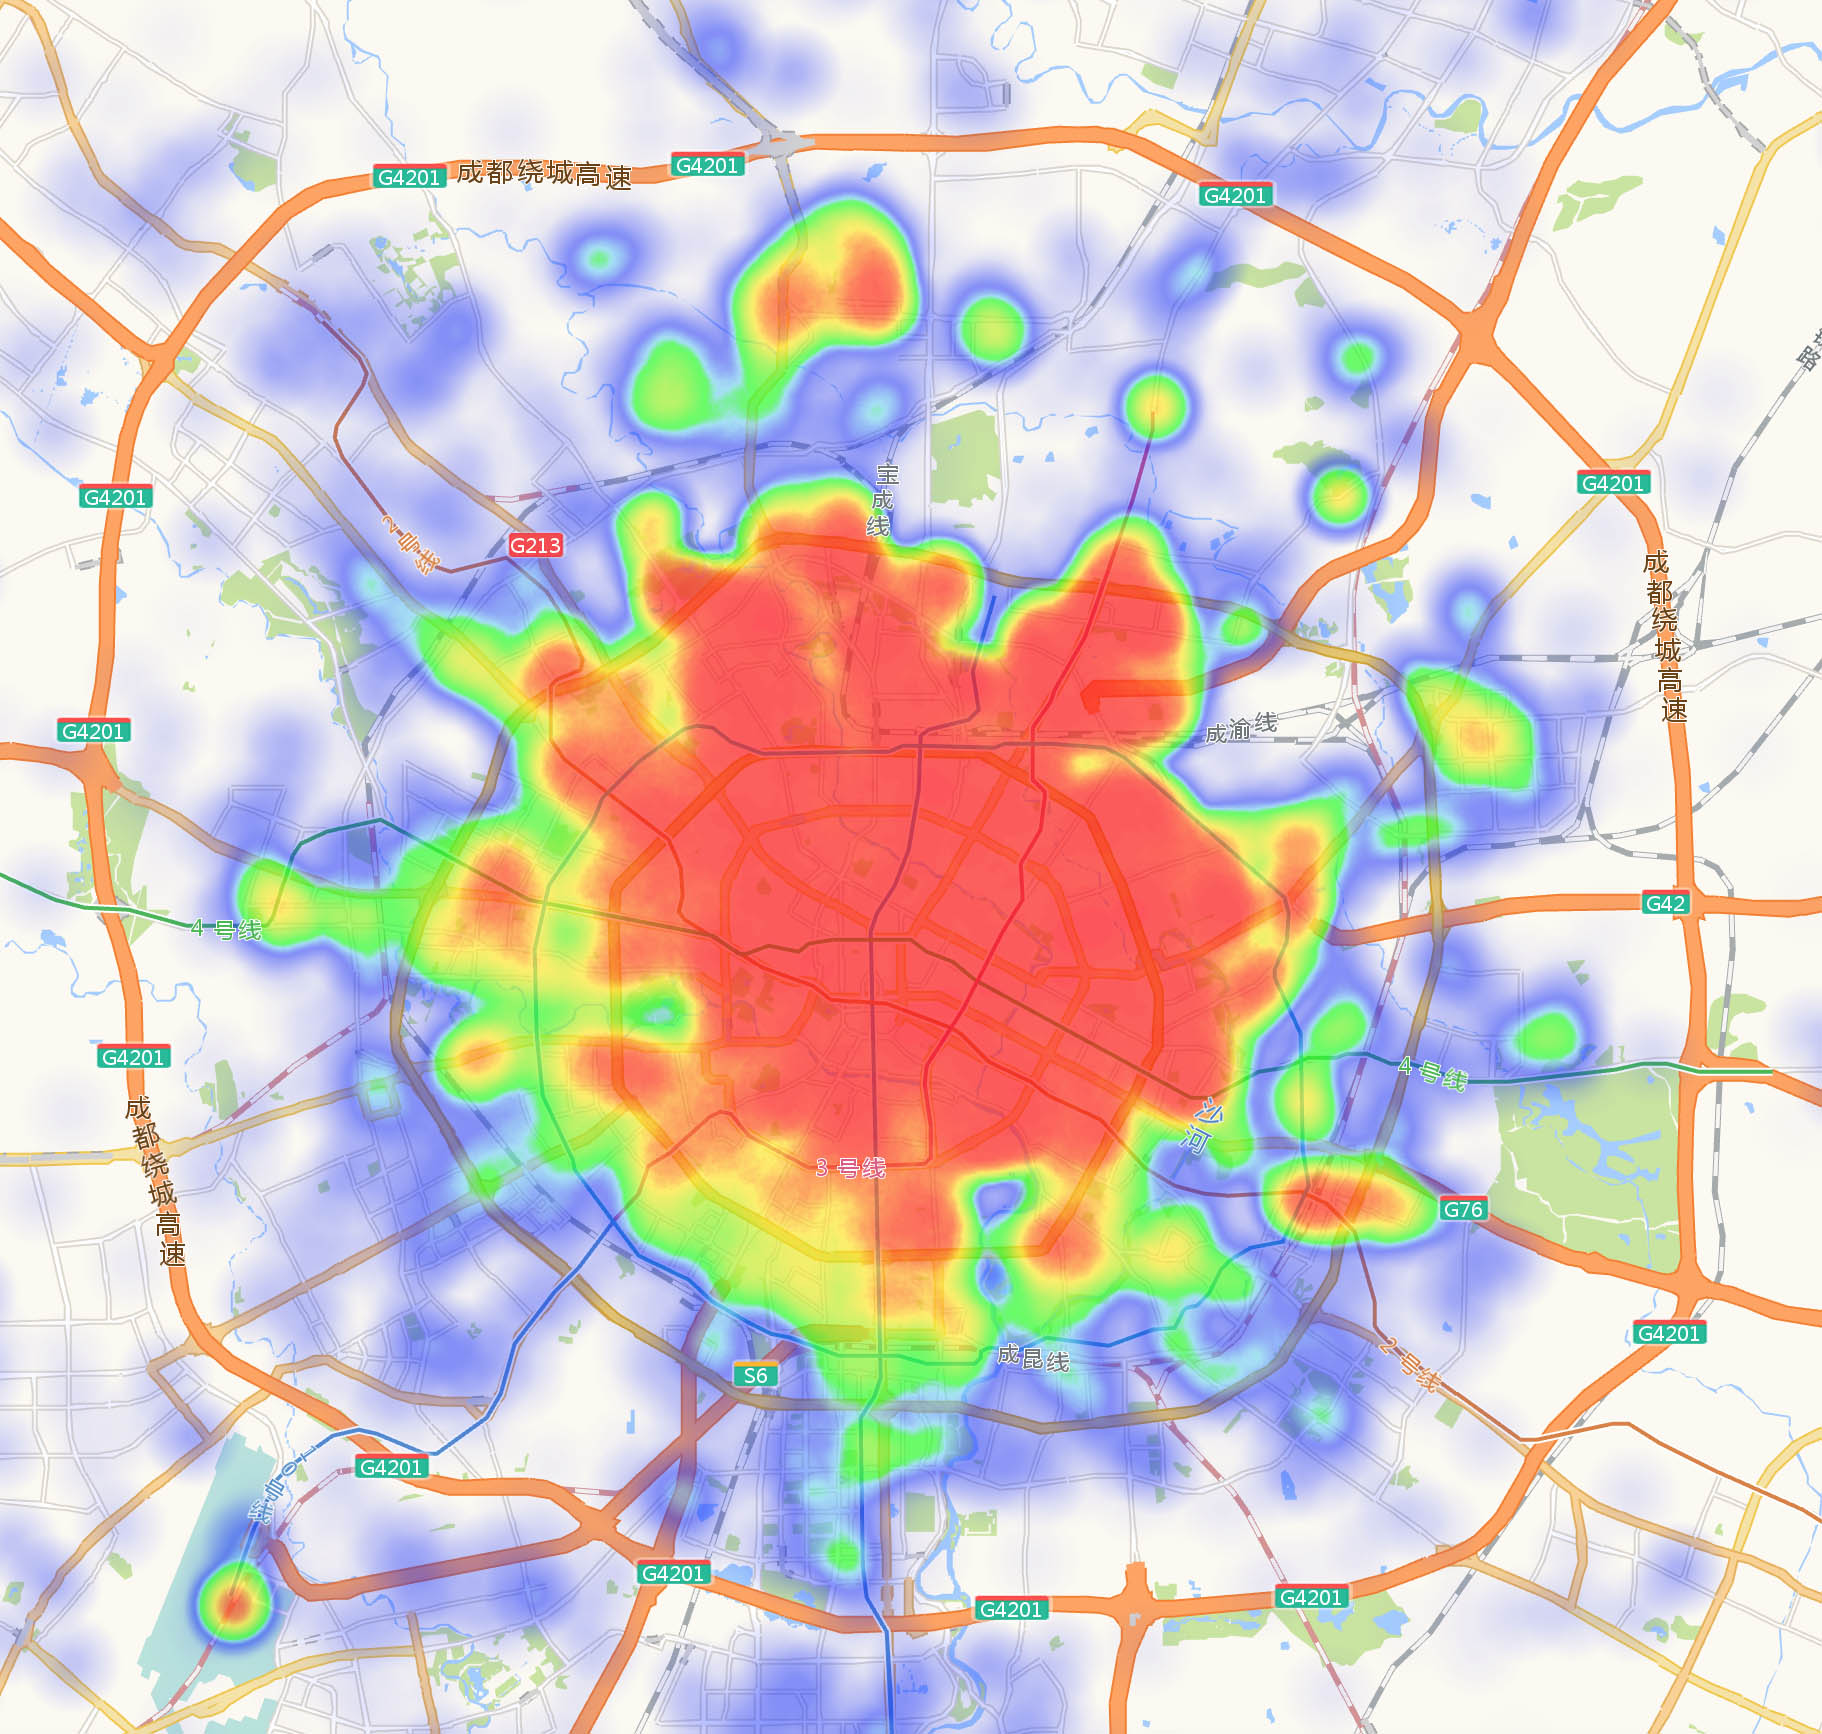
\includegraphics[width = 15em]{start.jpg}
		\caption{Heat Map of Origins}
	\end{minipage}
	\begin{minipage}[t]{0.4\textwidth}
		\centering
		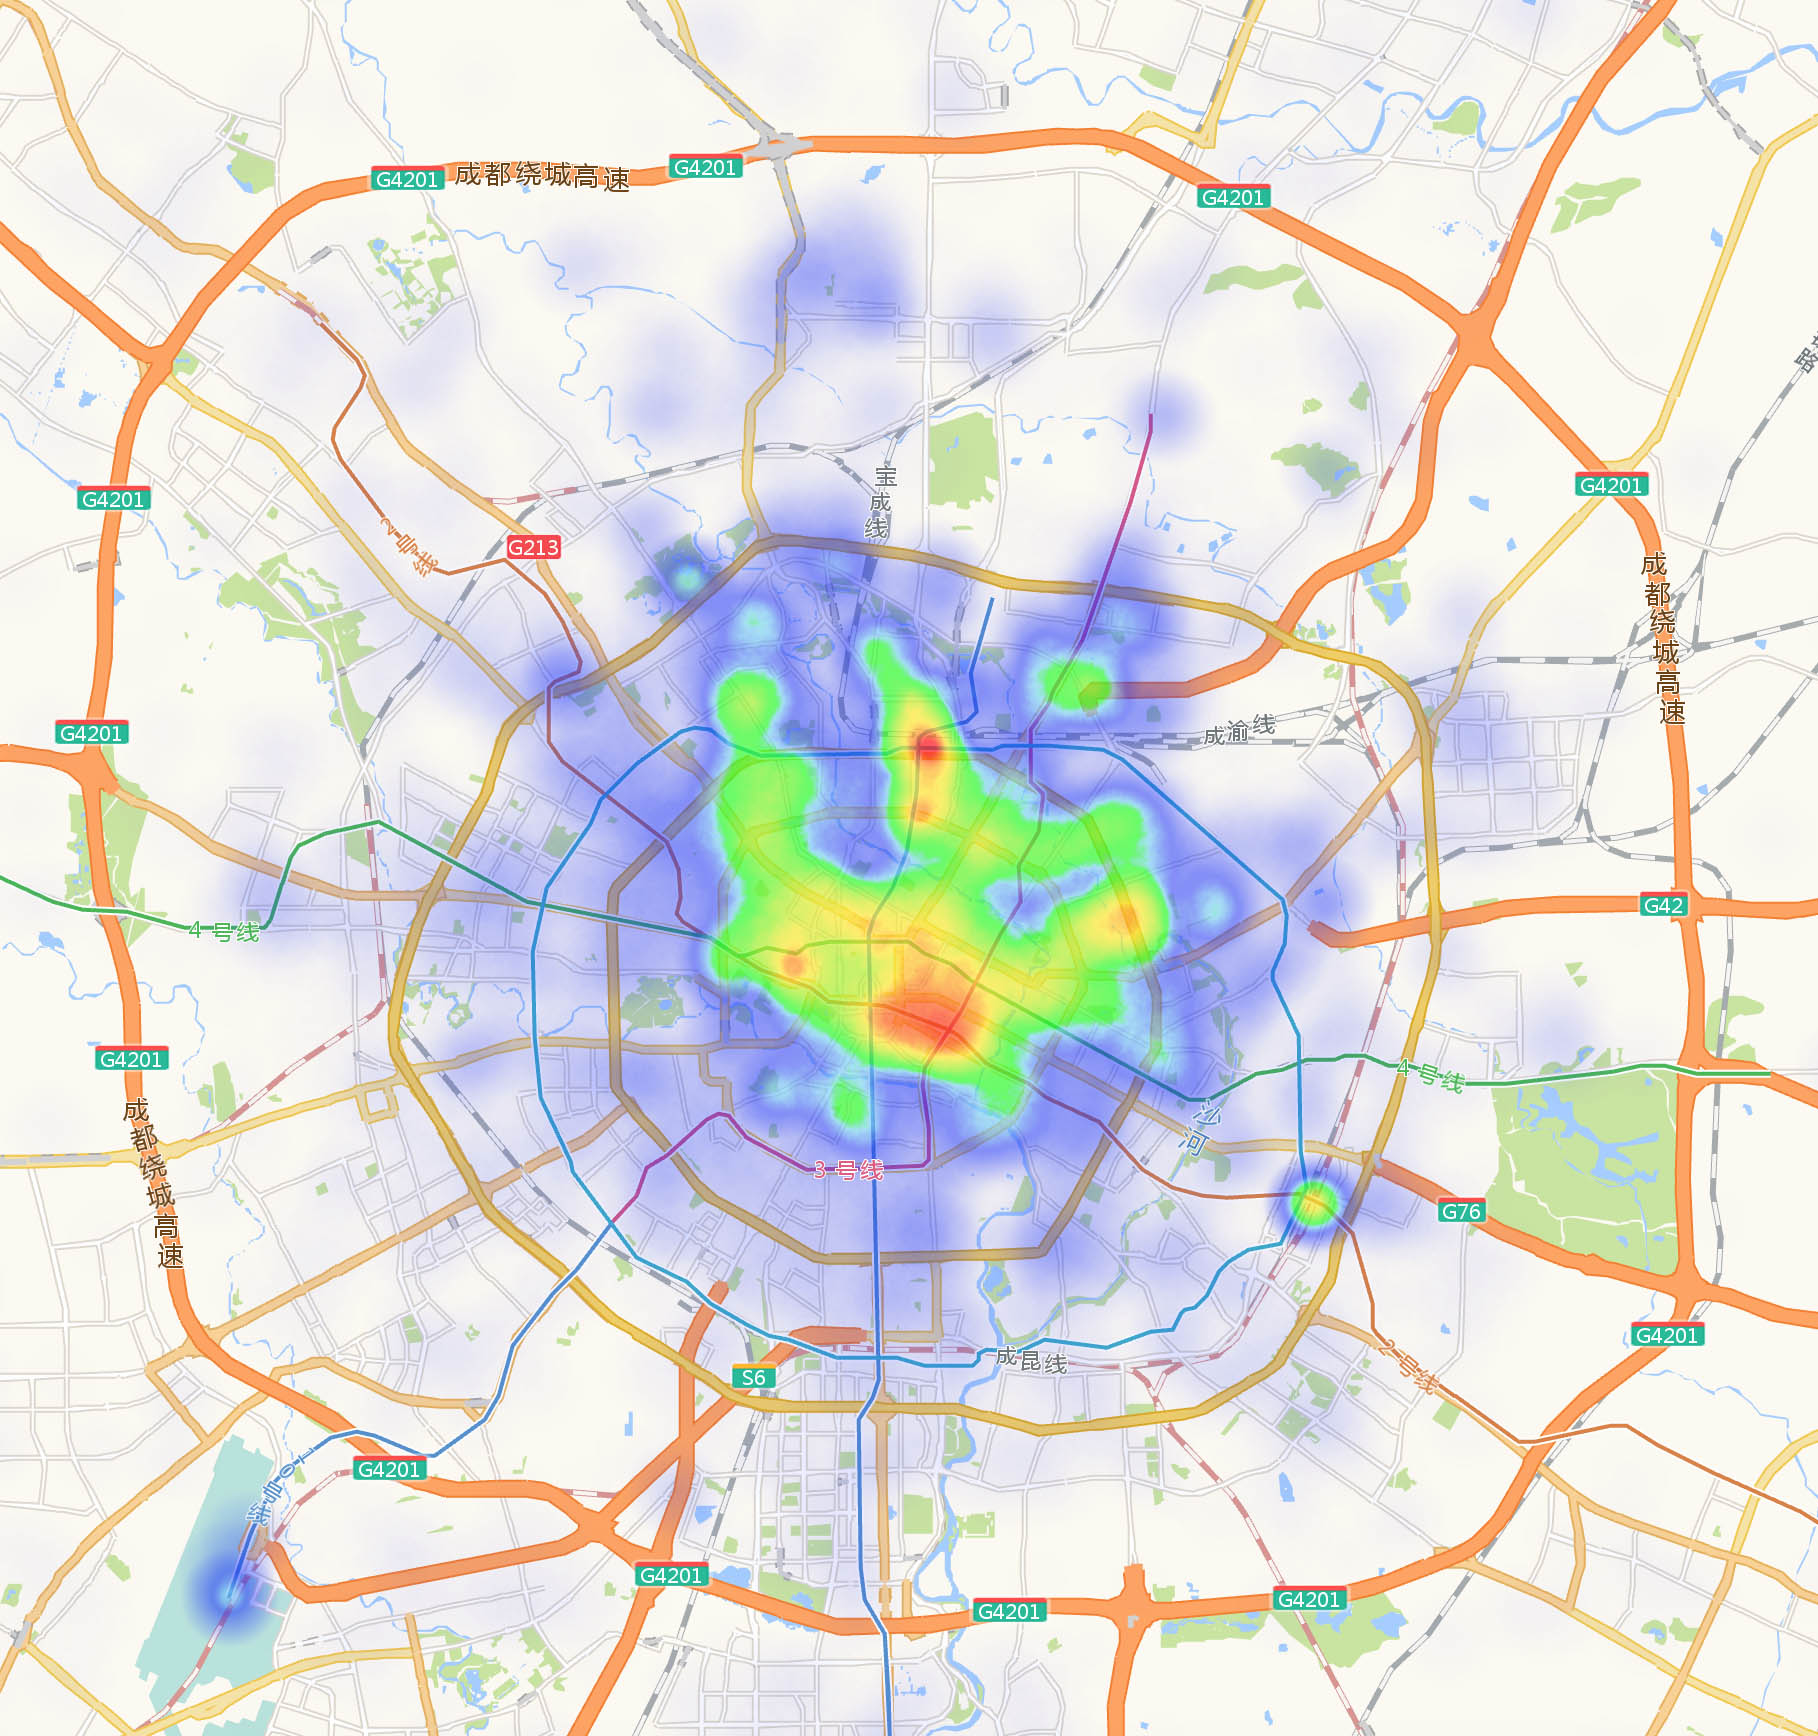
\includegraphics[width = 15em]{end.jpg}
		\caption{Heat Map of Destinations}
	\end{minipage}
\end{figure}

\begin{center}
	\textbf{III. Distribution Optimization}
\end{center}
\qquad After we use \emph{K-means} to get clusters of customers and cabs, we just see them as \emph{hubs}. A \emph{hub} is a site where customers and cabs around around could go and wait there for picking up \emph{$($ or waiting for next customer $)$}.

\qquad First optimization we will make is on the distribution system. Currently the distribution system is just fetching the nearest car around where the customer places the order. It is good for both the customer and the cab driver because it will make them both very efficient. However, in a larger scale, it is not so efficient. That the distance between the customer and the cab is whether 2 or 3 kilometers does not matter so much compared with the cab speed. Based on this, we may distribute a little farther but more vacant cabs to the customer ,and distribute nearer ones to where cabs are more urgently needed. It will cost both customers and drivers a little more time \emph{$($ on average 1 or 2 minutes for 1 or 2 extra minutes $)$}, but for the whole sector \emph{supply-demand} balance will be neutralized more.

\qquad From this point of view, I form a new distribution system, which takes two factors into consideration:
\begin{enumerate}
\item Supply-Demand in the sector of the cab
\item Distance to the customer
\end{enumerate}
we will finally calculate a \emph{"score"} for each cab. Sorted by the \emph{score}, we will pick up the most suitable one for the customer.

\qquad Based on this theory, we work out two methods to work out appropriate formula to calculate a score.
\\\\
\textbf{1. Manually Set Formula}

\qquad Based on observation of the whole dataset, we calculate the \emph{Supply-Demand} ratio and the distance between each cab and the customer. We think the \emph{Supply-Demand} ratio has higher prior than distance, since this will make only a couple of minutes longer when the difference is 1 or 2 kilometers.

\qquad After comparison, we think this formula works best:
\begin{displaymath}
	Score = 10^{Supply-Demand\ ratio^2-1}+100^{threshold\ distance - distance}
\end{displaymath}
In the formula, \emph{threshold distance} is the maximum appropriate distance between the cab to be dispatched and the customer. If distance between the customer and the cab goes beyond this threshold value, it is not very suitable, but it is acceptable if there is no nearer cabs around.

\qquad We also set two special occasions for distance factor. If the distance is smaller than \emph{minimum distance}, which could be set manually\emph{$($ by default it is 0.5 kilometer $)$}, the cab will directly get dispatched since it is so near that it costs almost nothing for this cad to pick up the customer. In contrast, if the distance is larger than \emph{maximum distance}, which could also be set manually\emph{$($ by default it is 4 kilometers $)$}, the cab will be excluded from the cab waiting list directly, since the cost for pickup
is far from satisfaction.

\qquad To test this formula, we assume that we call a cab on 1191 random sites in city center, the distance distribution is:

\begin{figure}[htbp]
	\centering
	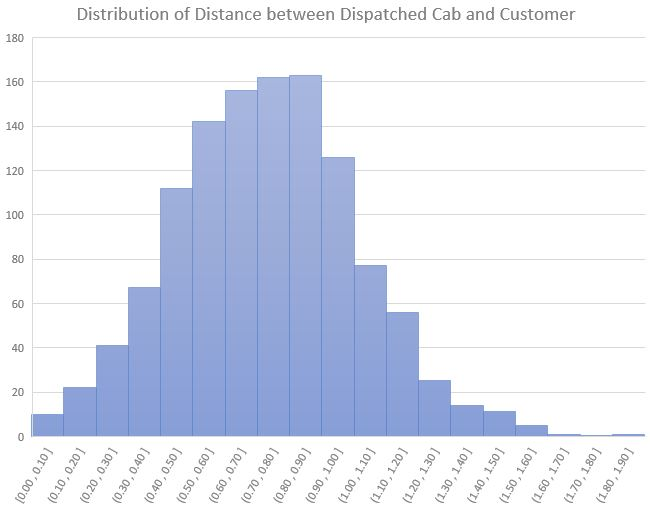
\includegraphics[width = 30em]{Distribution.JPG}
	\caption{Distribution of Distance between Dispatched Cab and Customer Using Manually Set Formula}
\end{figure}
%distribution picture here

\qquad The distribution is very normalized. On average, the distance between the dispatched cab and the customer is 0.786 kilometer, which is acceptable.
\\\\
\textbf{2. Formula from Supervised Learning}

\qquad Formula gotten from the first method works, but after all it is manually decided, which is not very reasonable. To make it more reliable and scientific, we use supervised learning to get a formula more reliable and scientific way.

\qquad First, we randomly take a coordinate as the customer location \emph{$($ \ang{104.0545;;}N, \ang{30.7116;;}E $)$}. Then we filter out suitable cabs, which are from \emph{minimum distance} to \emph{maximum distance} around. In total we have in total 2279 hubs meeting our requirement. Sorted by \emph{Supply-Demand} ratio, we give each of the hub a score manually, which show our preference for each hub.

\qquad After giving each cab hub a score, we start to get a general formula using supervised learning.

\qquad For supervised learning, we follow:
\[
  \begin{split}
	h_\theta (x) &= {\theta}_0 + {\theta}_1 x_1 + ... + {\theta}_n x_n\\
    &=x^{T} \theta
  \end{split}
\]
where each \(x_i\) is a feature deciding the value of function \(h(x)\). \(h_\theta(x)\) means the final function we get is only from features of \(\Theta\), which may have some bias with real \(h(x)\).

\qquad In this project, we have two features deciding the final score: \emph{Supply-Demand} ratio and distance from the customer. Therefore, let function \(h(x)\) be final score:
\begin{displaymath}
	h_\theta(x)=\theta_0 + \theta_1 x_1 + \theta_2 x_2
\end{displaymath}
where \(x_1\) represents the \emph{Supply-Demand} ratio factor and \(x_2\) represents distance factor. \(\theta_0, \theta_1, \theta_2\) are all constants making the final score reliable.

\qquad Just like the first method, \emph{Supply-Demand} ratio factor is more important than distance factor, so we choose more \emph{'dominant'} function for \(x_1\) than \(x_2\). For simplicity, define \(x_1 = r^2\) and \(x_2 = \ln(d)\), where \(r\) represents \emph{Supply-Demand} ratio and \(d\) represents distance between the cab and the customer.

\qquad Having gotten scores, distances and demand for each cab, we just do a little Linear Algebraic calculation. This method is also known as \emph{linear regression}:
\[
	\begin{split}
		X^T \theta &= H_\theta\\
        X^{TT} X^{T}\hat{\theta} &= X^{TT} H_\theta\\
        XX^{T}\hat{\theta} &= XH_\theta\\
        \hat{\theta} &= {(XX^{T})}^{-1}XH_\theta
	\end{split}
\]
where the last raw of matrix \(X\) will be 1 since \(\theta_0\) is \emph{constant parameter}.

\qquad Directly calculate inverse of \(XX^{T}\) using determinants is rather slow. Suppose we have \(n\times n\) matrix, using \(Crammer's\ Rule\), time complexity is \(\Theta(n^3)\) since we need to calculate \(det (B_i)\) each time, which needs to solve two \(n\times n\) matrices' multiplication. We use \(SVD\) to optimize the procedure. Though time complexity is still \(O(n^3)\), runtime has an improvement. This is because \emph{SVD} saves some steps during calculation. We plan to use \emph{Coppersmith-Winograd algorithm} to boost it more, which has \(O(n^{2.38})\) time complexity. However, till the hand-in deadline we have not implemented it correctly.

\qquad Getting \(\hat{\theta}\), just like the first method, we randomly choose 1139 point to call a "cab". Distribution of distance between cabs and customers is below:
\pagebreak

\begin{figure}[htbp]
	\centering
	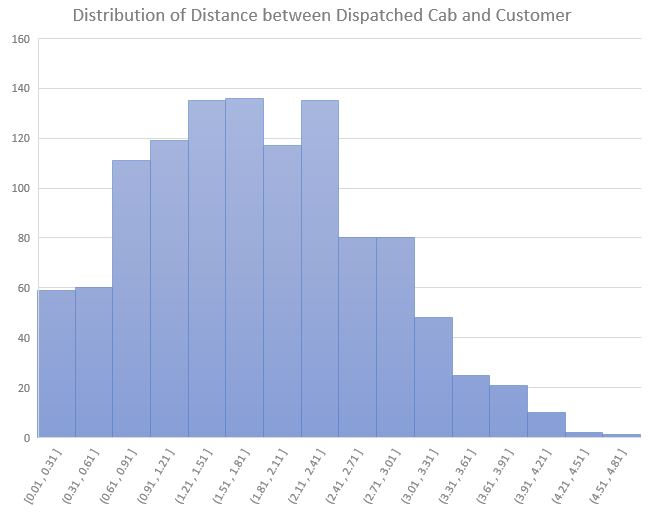
\includegraphics[width = 35em]{Distribution_2.JPG}
	\caption{Distribution of Distance between Dispatched Cab and Customer Using Supervised Learning}
\end{figure}
%insert a figure

\qquad Compared with Manual Method, average distance becomes larger and variance is larger too. But still it is acceptable. It is highly possible that functions we choose for \(x_1\) and \(x_2\) are too arbitrary, we need more trials to make it more reliable. Supervised Learning itself also causes inaccuracy. If permitted, we will use \(NN-algorithms\) to make it more flexible and accurate.

\begin{center}
	\textbf{IV. Real-Time Bonus}
\end{center}

\qquad Nevertheless, distribution optimization just makes \emph{Supply-Demand} ratio as balanced as possible at the last time. If there is a relatively large sector where cabs are in urgent short, however distribution is optimized, customers will not all be satisfied. To solve this, we need to motivate cab drivers to drive where cabs are urgently needed. Bonus is the best to motivate them.

\qquad In fact, \emph{Didi} itself has pushed forward bonuses for orders from specified areas, such as \emph{Zhangjiang} in \emph{Pudong}. However, it updates every three days or even every week. It is complained by many drivers because of its lagging. We aim to design a real-time bonus model for \emph{Didi} so that bonus will be much more efficient than the current one.

\qquad According to \emph{Uber Mini Project}, they form a model of bonus:
\begin{displaymath}
Bonus = Bonus\ Base\ \times\ Variance^{1-Supply-Demand\ Ratio}  
\end{displaymath}
It provides a basic bonus and then relate it with urgency of supply and demand. To be more detailed, we form the formula to:
\begin{displaymath}
Bonus = k_b \times {k_v}^{\frac{c}{t}}
\end{displaymath}
where \(k_b\) is Bonus base constant, \(k_v\) is variance constant, \(t\) is the number of available cabs and \(c\) is the number of customers.

\qquad First, we define\emph{urgent hubs} as those who has fewer cabs than customers in the sector we set. And \emph{lacking hubs} as those who has less than a certain number of cabs left for possible customers to take. The certain number is defined as \(Theshold Cab Left Number\). Only this two kinds will need bonus to motivate vacant cabs to meet customers' needs. Due to difference on urgency, two kinds of bonus hubs will have different

\qquad Cab drivers we give bonus to is also a question. We take the following method: we set maximum distance for drivers to get bonus. Only those within maximum distance will be targets of bonus. Then, we will calculate the \emph{supply-demand} ratio for each cab hub, only those who are neither \emph{urgent hubs} nor \emph{lacking hubs} will be valid for bonus.

\qquad Finally, for those who are valid for bonus, we will also give compensation based on distance from the initial cab hub to \emph{urgent hubs} or \emph{lacking hubs}.

\qquad Taking all factors into consideration, we work the final formula:
\begin{displaymath}
	Bonus = u\times k_b \times {k_v}^{\frac{c}{t}} + cpk\times d
\end{displaymath}
where \(u\) means urgency of the bonus hub. The more urgency it is, the larger \(u\) is. \(cpk\) means \emph{Compensation per kilometer}. In fact, it has already existed to compensate cab drivers from current location to pickup location. For example, in \emph{Shanghai} it is 0.8 \emph{yuan} per kilometer \emph{(told by a Didi driver)}.

\begin{center}
	\textbf{V. Hub Deployment Improvement}
\end{center}
\qquad From Fig.1, it is very obvious that pickup locations have a very regular distribution. In future, we could only allow customers to get a cab in regulated hubs.

\qquad Take \emph{Jinke Road Subway Station} around as an example:
\begin{figure}[htbp]
	\centering
	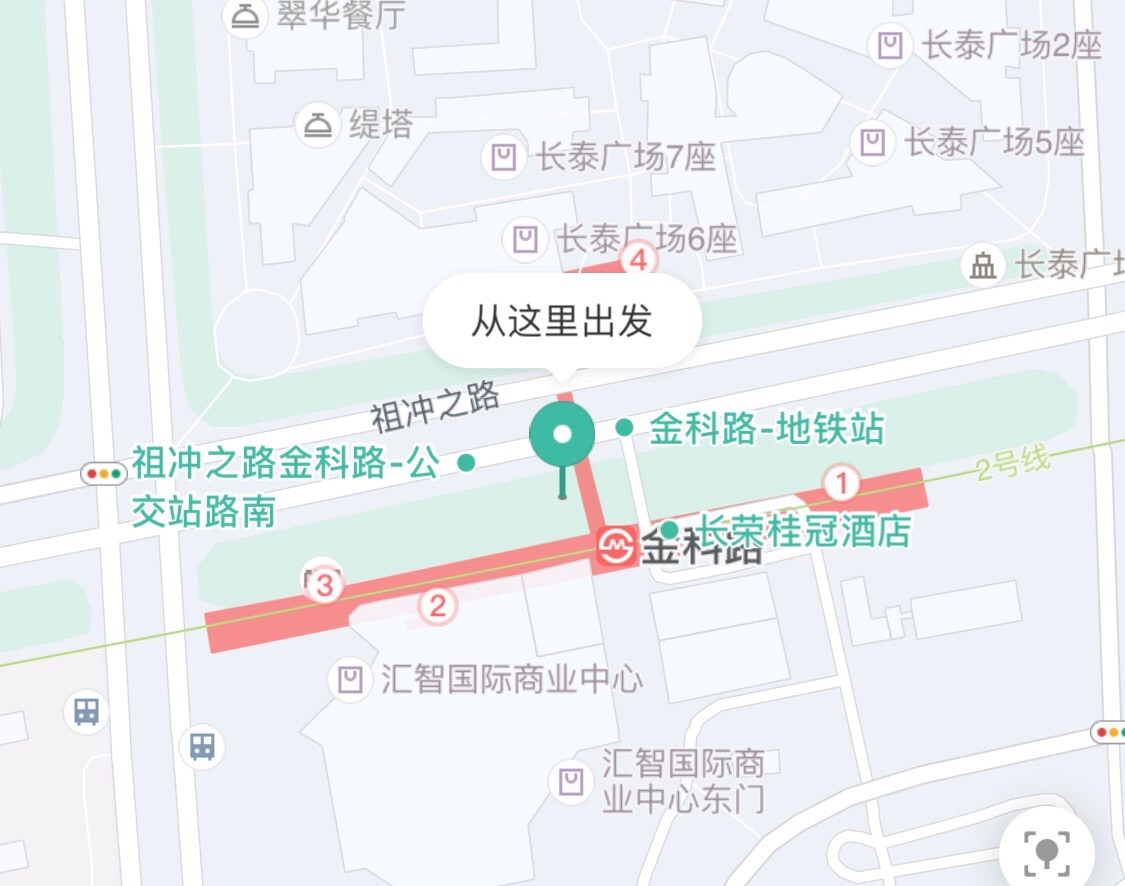
\includegraphics[width = 35em]{JinkeRoad.jpg}
	\caption{Jinke Road Subway Station \emph{(from Didi Chuxing App)}}
\end{figure}

From figure 5, there are 3 pick up hubs for customers, but from our using experience, the pickup location in the middle and on the south side is very inconvenient for both cab drivers and customers. A traffic accident occurred once near \emph{Jinke Road-Subway Station} pickup hub just because of picking up a customer on that hub. In the future, \emph{Didi} should consider making surveys around the busy sectors and allow only safe hubs to pick up and drop off customers. Not only will traffic be safe, it will be convenient for both customers and cab drivers.

\clearpage
\bibliographystyle{plain}
\bibliography{reference}

\end{document}
